\documentclass[12pt]{article}
\usepackage[top=2cm, bottom=3cm, left=2.5cm, right=2.5cm]{geometry}

\usepackage{amssymb,amsmath,amsfonts,eurosym,geometry,ulem,graphicx,caption,color,setspace,sectsty,comment,footmisc,caption,pdflscape,subfigure,array,hyperref}
\usepackage[round]{natbib}
\usepackage{amsthm,amscd}
\usepackage{amsmath}
\usepackage{lastpage}
\usepackage{enumerate}
\usepackage{fancyhdr}
\usepackage{mathrsfs}
\usepackage{graphicx}
\usepackage{blindtext}
\usepackage{hyperref}
\hypersetup{hidelinks}
\usepackage{setspace}
% \doublespacing
\usepackage{booktabs}

\title{ Predicting Geriatric Depression Using \\ Machine Learning Models}
\date{}
\author{Ruibing Su}

\begin{document}
\maketitle

% ***************************************************
% ***************************************************
\section{Introduction}
\par Geriatric depression is a mental health condition in older adults. It is a mood disorder in which feelings of sadness, loss, anger, or frustration interfere with daily life for weeks or longer. Geriatric depression has serious negative effects on the elderly. \cite{alexopoulos2009research} pointed out that geriatric depression not only causes suffering and involves suicide risk; it also increases medical comorbidity and disability among elderly individuals. Although depression in older adults is a widespread problem, it is often not recognized or treated. \cite{onishi2006comparison} found that clinicians tend to underestimate the presence of depression because depressive symptoms are often assumed to be a part of normal aging, not related to the disease of depression. Besides, geriatric depression is also frequently masked by physical symptoms and can be easily ignored by family members.

\par The population of China is aging rapidly due to a longer life expectancy coupled with a dramatic decline in fertility rates. According to the UN standards, a country is an aging society if the share of the population over 60 exceeds 10 percent of the whole population. China’s census data shows that the share was 10.46 percent in 2000, 13.26 percent in 2010, and 18.80 percent in 2020. Given the total population of China increased to 1.41 billion in 2020, the population aged 60 and over in China has increased to 265 million. \cite{zhang2012prevalence} stressed that among these older people in China, many suffer from a wide range of problems, including physiological dysfunction, chronic diseases, and feelings of loneliness because of far-away children. These changes often lead to inferiority and fear and, if not taken care of, can lead to depression. The early intervention of depression is premised on the identification of depression risk in the elderly. So the huge demographic shift presents new challenges for public health policymakers.

\par Depression is an important topic in both economics and machine learning. In economics, researchers are more interested in the causal relationship between depression and public policies. For example, \cite{chen2019does} found social pension expansions significantly reduce the geriatric depression risk among the elderly. On the other side, In machine learning, researchers are more concentrated on the accuracy of prediction models. A number of recent studies used clinical information to predict depression risks. For example, \cite{trinh2011using} used electronic medical records to determine the diagnosis of depression. These algorithms have excellent performance but are not practical in China. The elderly, especially those living in rural areas, still have difficulty accessing regular and detailed medical examinations to build clinical records.

\par The goal of this project is to predict geriatric depression among the elderly using social survey data, which are easy to collect in China. In this project, 5 models, including Logistic Regression, KNN, Random Forest, Adaboost, and Multilayer Perceptron (MLP), are built, trained, and tested on the China Health and Retirement Longitudinal Study (CHARLS) dataset. Recall, ROC, and AUC are used to evaluate the performance of the 5 models. The results show that Logistic Regression, Random Forest, and Adaboost have higher recall and AUC, which means that a decision system based on the three models may be valuable for the early diagnosis and intervention of geriatric depression.

% ***************************************************
% ***************************************************
\section{Data}
% ***************************************************
\subsection{Data Source}
\par The data used in this project come from the China Health and Retirement Longitudinal Study (CHARLS), which collects a high-quality nationally representative sample of Chinese residents ages 45 and older to serve the needs of research on the elderly. The survey was conducted by Peking University in 2015, covering about 13000 respondents in 450 communities.

\par CHARLS includes a rich set of data on economic standing, physical and psychological health, demographics and social networks of aged persons. The dependent variable in the project is whether the respondent is depressed or not, and the independent variables can be generally categorized into three groups: demographics and living conditions, activities of daily living, and physical health. Depression is constructed based on the Epidemiologic Studies-Depression scale (CESD) scale, which is a self-report rating scale that is designed to measure current symptoms of depression. Demographics and living conditions include gender, age, marriage status, education level, employment status, whether living in rural areas, number of living sons, number of living daughters, whether living with children, number of individuals in the household, total value of durable assets, amount of money transferred to children last year, amount of money received from children last year, and province.\footnote {Durable assets include: Refrigerator, Washing machine, TV, Computer, Stereo system, Camera, Air conditioner, Mobile phone, Furniture,  Music instrument,  Valuable decorations, ornaments, and vases,  Treasures and precious metal,  Antiques, valuable paintings and calligraphic work and other artistic work.} Information on activities of daily living includes whether the respondent reports ever smoking, whether the respondent has had an alcoholic beverage in the last 12 months, whether the respondent participates in any social activities, whether the respondent has difficulty in dressing, eating, making phone calls, managing money and taking medication, and the respondent’s logical ability and memory ability. \footnote { The social activities include: interacting with friends, playing ma-jong, chess, or cards, going to a community club, going to a sporting event, participating in a social group, taking part in a community-related organization, taking part in voluntary or charity work, and attending an educational or training course.} Information on physical health includes whether the respondent reported having hypertension, diabetes, cancer, lung diseases, heart problems, stroke, arthritis, dyslipidemia, liver diseases, kidney diseases, and digestive diseases.


% ***************************************************
\subsection{Exploratory Data Analysis}
First, I analyzed the missing data pattern of the dataset. The data set has 12676 observations and 40 features. Table \ref{Data_Missing} shows the missing rates of all the variables. From the table, it is shown that the maximal missing rate is not greater than 7\%. Given that each variable only contains a small number of missing values, I imputed all missing values with the median of the corresponding variable.

\begin{table}[htbp]
  \centering
  \caption{Missing Rate} \label{Data_Missing}
     \scalebox{0.7}{
    \begin{tabular}{cccccc}
    \toprule
    \toprule
    Variable  & \# Missing   & Missing Rate   & Variable  & \# Missing   & Missing Rate \\
    \midrule
    Depression   & 0     & 0\%   & Diff\_phone  & 54    & 0\% \\
    Male     & 0     & 0\%   & Diff\_money & 75    & 1\% \\
    Age       & 0     & 0\%   & Diff\_medicine  & 31    & 0\% \\
    Married    & 0     & 0\%   & Smoke  & 7     & 0\% \\
    L\_Edu   & 15    & 0\%   & Alcohol  & 8     & 0\% \\
    M\_Edu  & 15    & 0\%   & Social\_Acti  & 1     & 0\% \\
    H\_Edu  & 15    & 0\%   & Logic   & 70    & 1\% \\
    Working  & 154   & 1\%   & Memory  & 393   & 3\% \\
    Rural & 0     & 0\%   & H\_bpressure   & 693   & 5\% \\
    Son    & 0     & 0\%   & Diabetes   & 729   & 6\% \\
    Daughter  & 0     & 0\%   & Cancer     & 661   & 5\% \\
    Coresd  & 0     & 0\%   & Lung    & 636   & 5\% \\
    HHres  & 0     & 0\%   & Heart   & 693   & 5\% \\
    Durable  & 101   & 1\%   & Stroke     & 614   & 5\% \\
    MoneytChild  & 113   & 1\%   & Arthritis    & 650   & 5\% \\
    MoneyfChild  & 113   & 1\%   & Dyslipidemia   & 934   & 7\% \\
    Province  & 0     & 0\%   & Liver   & 683   & 5\% \\
    Diff\_bath  & 228   & 2\%   & Kidney  & 681   & 5\% \\
    Diff\_dress & 215   & 2\%   & Digest  & 632   & 5\% \\
    Diff\_eat  & 215   & 2\%   & Asthma    & 639   & 5\% \\
    \bottomrule
    \end{tabular}}
    \vspace{-0.5em}
\end{table}%


Second, outliers are deleted from the data. By definition, only three variables (total value of durable goods, amount of money transferred to children last year, amount of money received from children last year) does not have an upper bound, which may result in outlier problems. Figure \ref{Impute_Durable_Box}, \ref{Impute_MoneytChild_Box}, and  \ref{Impute_MoneyfChild_Box}  in Appendix give the box plots of the three variables. The three plots demonstrate that the minimum, 25th percentile, median, and 75th percentile values of the three variables are all much smaller than their maximum values. For further investigation, I computed the values of the 90-100 percentile of the three variables, as shown in Table \ref{Data_Missing}. There is an anomalous gap between the 99 and 100 percentiles. Considering that these abnormal data might come from respondents' fabrication or interviewers' recording errors, I deleted all the observations with at least one of the three variables above the 99 percentile. Specifically, 393 observations are deleted, and the remaining dataset's size is 12283.

\begin{table}[htbp]
    \centering
    \caption{Percentail Distribution}   \label{Money_Percentail}
       \scalebox{0.9}{
      \begin{tabular}{cccc}
      \toprule
      \toprule
            & Value of Durable Goods & Money Transferred to Children & Money Received from Children \\
      \midrule
      90\%  & 14000 & 13500 & 11300  \\
      91\%  & 16000 & 14600 & 12200  \\
      92\%  & 20000 & 16000 & 13150  \\
      93\%  & 20000 & 18500 & 14337  \\
      94\%  & 22000 & 20000 & 15800  \\
      95\%  & 26000 & 22000 & 17700  \\
      96\%  & 30000 & 25000 & 20500  \\
      97\%  & 40000 & 30000 & 24275  \\
      98\%  & 50000 & 35795 & 29900  \\
      99\%  & 100000 & 50000 & 46150  \\
      100\% & 800000 & 750000 & 739500  \\
      \bottomrule
      \end{tabular}}
  \end{table}%

Table \ref{Data_Describe} in Appendix gives the descriptive statistics of the dataset. Overall, the prevalence of depression is about 9\%, the average age of all the respondents is 61, the average value of respondents’ durable assets is $\yen$4,132, the average amount of money transferred to children last year is $\yen$3,714, and the average amount of money received from children last year is $\yen$4,686.

Figure \ref{Demo_Depression_Clear} in the Appendix provides a correlation heatmap of the data, demonstrating the correlation between depression, demographic and living condition variables. It is observed that: geriatric depression is more prevalent in males; depression is positively correlated with age; the proportion of depression is higher among people who live alone and people who live in rural areas. Figure \ref{ADL_Depression_Clear} in the Appendix provides another correlation heatmap, which demonstrates the correlation between depression and activities of daily living. The figure presents that: various behavioral disorders, including having difficulty in bathing, dressing, eating, making a phone call, managing money, and taking medication, are significantly positively correlated with depression; lifestyle habits, such as smoking, drinking, and participating in social activities, have a negative correlation with depression; in addition, logic ability score and memory ability score are negatively correlated with depression. Figure \ref{Diease_Depression_Clear} depicts the correlation between depression and physical health conditions. The figure shows that almost all diseases are positively correlated with depression. In fact, the advantage of the CHARLS dataset is that it contains complete and accurate information on respondents’ daily activities and health conditions.

% ***************************************************
% ***************************************************
\section{Models and Results}
% ***************************************************
\subsection{Models}
\par In this section, I will introduce the evaluation metrics and the models used in this project, the optimal parameters selected for each model, and the performance of each model.

\par Before building the model, I first standardized the dataset to improve the performance of the models, and I also used one hot encoding to convert province into a group of binary variables.

\subsubsection{Evaluation Metrics}
Performance metrics are a part of every machine learning pipeline. It measures the performance of machine learning models. It should be emphasized that throughout this project, the performance of the models is evaluated based on recall and the receiver operating characteristic curve (ROC). 
\[
    Recall = TPR = TP/(TP+FN)
\]
\[
    FPR = FP/(FP+TN)
\]
\[
    Accuracy = (TP+TN)/(TN+TP+FN+FP)
\]

Here, true negatives (TN) and true positives (TP) indicate the number of the elderly that were accurately identified as depressed and not depressed, respectively; false negatives (FN) and false positives (FP) indicate the number of the elderly that were inaccurately identified as not depressed and depressed, respectively.

Usually, machine learning models are evaluated using accuracy, which is a useful metric to quantify a model's performance in general. However, when it comes to depression detection, we are more concerned about the accuracy of the model in actual patients. Especially when the data is unbalanced, accuracy is misleading. In contrast to the accuracy metric, recall provides useful information about the fraction of positive observations that were correctly identified out of the total pool of positives.

Receiver operating characteristic (ROC) graphs are also a useful tool to select models for classification tasks based on their performance with respect to the false positive rate (FPR) and true positive rate (TPR). The TPR and FPR along the ROC curve are computed by shifting the decision threshold of the classifier. The diagonal of a ROC graph can be interpreted as random guessing, and classification models that fall below the diagonal are considered as worse than random guessing. A perfect classifier would fall into the top-left corner of the graph with a TPR of 1 and an FPR of 0. With the ROC curve in hand, the area under the ROC curve (AUC) can be computed. AUC characterizes the performance of a classification model.

% ***************************************************
\subsubsection{Logistic Regression}
\par Logistic regression is a classification model suitable for the depression detection task. Logistic regression is a generalized linear model. Let $p$ stand for the probability of the positive target, i.e., depression = 1. Then $p$ is modeled as:
\begin{align*}
p &= \frac{1}{1+e^{-z}} \label{Logistic_function}\\
z &= \omega'x+b
\end{align*}
where $x$ is a vector of independent variables, and $b$ is a vector of corresponding coefficients. Logistic regression has many advantages. For example, logistic regression is efficient to train and easy to interpret; Logistic regression also makes no assumptions about distributions of classes in feature space. On the other side, logistic regression also has disadvantages. It assumes the relationship between log odds and independent variables is linear and can only construct linear boundaries.

Regarding optimal parameters, since the geriatric depression detection is a typical binary classification problem and the structure of the logistic algorithm itself is relatively simple, I did not add regularization to the model.

% ***************************************************
\subsubsection{k-Nearest Neighbor(KNN) classifier}
KNN is a non-parametric model. It does not learn a discriminative function from the training data but memorizes the training dataset instead. The basic idea of KNN is to find the k examples in the training dataset that are closest (most similar) to the point that we want to classify based on a distance metric and then assign the class label by a majority vote among the target’s k nearest neighbors. k is a critical hyperparameter of the model. If k is too small, the model will likely overfit the training data; if k is too large, the model will tend to underfit the training data. The right choice of k is crucial to finding a good balance between overfitting and underfitting.

Generally, distance metrics can be written as follows:
\begin{align*}
L_{p}\left(x_{i}, x_{j}\right)=\left(\sum_{l=1}^{n}\left|x_{i}^{l}-x_{j}^{l}\right|^{p}\right)^{\frac{1}{p}}
\end{align*}

\par $p=1$ corresponds to the Manhattan distance metric; and $p=2$ corresponds to the Euclidean distance metric. From the equation, it can be seen that the relative scale of the independent variables affects the distance significantly. However, the relatively larger variables are not necessarily more important, so I normalized all the independent variables before building any model.
To determine the optimal parameters, I used the GridSearchCV function in sklearn. Based on the cross-validation algorithm, GridSearchCV gives the optimal parameters, k = 5 and p =2.


% ***************************************************
\subsubsection{Random Forest}
Random forest is a variant of the bagging algorithm. It can be considered an ensemble of decision trees. The basic idea is to average multiple decision trees that individually suffer from high variance to build a more robust model.

The random forest algorithm can be summarized in four simple steps: 1, randomly choose n examples from the training dataset with replacement; 2, train a decision tree using the bootstrap replica: at each node; 2.1, random select k features without replacement; 2.2, split the node using the feature that can maximize the information gain. 3. aggregate the prediction by each tree to assign the class label by majority vote. Random forest increases the degree of variation among the decision trees by attribute perturbation

Three critical hyperparameters in the random forest algorithm are the number of trees in the forest, n\_estimatorsint, the maximum depth of each tree, max\_depth, and the number of features to consider when looking for the best split, max\_features.

In the determination of the optimal parameters, GridSearchCV was employed using the training dataset. Because of the limitation of computation power, the three optimal parameters are generated one by one. To be more specific, I first searched for the optimal number of trees, with all other hyperparameters set as default. With the optimal n\_estimatorsint = 50 in hand, I then searched for the optimal maximum depth of each tree, and GridSearchCV shows the optimal max\_depth = 12. With n\_estimatorsint = 50 and max\_depth = 12, GridSearchCV gives the optimal max$\_$features = 10. It is noteworthy that a rigorous analysis should search for the three parameters simultaneously rather than this step-by-step method.

% ***************************************************
\subsubsection{Adaboost}
AdaBoost is a variant of the boosting algorithm. It can be viewed as an ensemble of weak classifiers, which only have a slight performance advantage over random guessing. The basic idea behind this algorithm is to let the weak classifier subsequently learn from misclassified training examples to improve the performance of the ensemble.

When building the Adaboost mode, I used a decision tree stump, DecisionTreeClassifier with max\_depth=1, as the weak learner. As above, GraidSearchCV is introduced to search for the optimal parameters, the number of weak classifiers, n\_estimators, and it gave that the optimal n\_estimators = 40.


% ***************************************************
\subsubsection{Multilayer Perceptron}
A multilayer perceptron is a fully connected multilayer feedforward artificial neural network. Similar to other feedforward neural networks, MLP contains three kinds of layers: input layer, hidden layer, and output layer, and each node in MLP has an activation function. There are four popular activation functions: the identity function, $f(x) = x$; the logistic sigmoid function, $f(x) = 1 / (1 + exp(-x))$; the hyperbolic tan function is $f(x) = tanh(x)$; and the rectified linear unit function $f(x) = max(0, x)$. Among them, the rectified linear unit function (ReLU) is more frequently used in the recent development of deep learning. One of the reasons is that ReLU can help mitigate the vanishing gradient problem.

In the determination of the optimal parameters, I mainly focused on the structure of the neural network and the activation function. Due to the limitation of computing power, the network is restricted to 4 hidden layers with no more than 400 neurons, and the GridSearchCV gave that the optimal hidden layer size is (200, 100, 50, 20) and the optimal activation function is ReLU. It is also worth mentioning that rigorous analyses should conduct optimal parameter searching in a larger parameter space.
% ***************************************************
\subsection{Results}
\par This section reports the performance of the 5 machine learning models (Logistic, KNN, Random Forest, Adaboost, and MLP) on the CHARLS dataset.
\subsubsection{Recall and efficiency}
First, recall is used to evaluate the performance of the 5 models. The experiment is set as follows: for each random state from 1 to 50: the dataset is split into an 80 percent training dataset and a 20 percent testing dataset according to the random state; all 5 models are trained on the training dataset and evaluated on the testing dataset. The results of the experiment are shown in Table \ref{Prediction_50}. The random forest model has the highest recall among the 5 models, and the logistic regression model has the second highest recall. Besides, the performance of the Adaboost model is better than the performance of the KNN model. The performance of MLP is disappointing. The recall of the MLP model is only about 39\%. Table 3 also gives the running time of the 5 models. It is evident that MLP is also the slowest model.
\begin{table}[htbp]
    \centering
    \caption{Performance of the 5 models} \label{Prediction_50}
       \scalebox{0.9}{
      \begin{tabular}{cccccccc}
      \toprule
      \toprule
            & Logit  & KNN   & RF &  Adaboost & MLP \\
      \midrule
      Run Time (s) & 1.98 & 15.67 & 10.56 & 26.39 & 474.85 \\
      \midrule
      Recall:  &        &        &        &         &       \\
      mean     & 0.6288 & 0.5173 & 0.6340 & 0.6083  & 0.3877\\
      std      & 0.0452 & 0.0549 & 0.0765 & 0.0502  & 0.0416\\
      min      & 0.5176 & 0.4098 & 0.4630 & 0.5217  & 0.2800\\
      25\%     & 0.6061 & 0.4827 & 0.5897 & 0.5761  & 0.3557\\
      50\%     & 0.6258 & 0.5150 & 0.6410 & 0.6049  & 0.3977\\
      75\%     & 0.6611 & 0.5533 & 0.6919 & 0.6435  & 0.4152\\
      max      & 0.7368 & 0.6567 & 0.7907 & 0.7059  & 0.4936\\
      \bottomrule
      \end{tabular}}
      \begin{flushleft}{
      Note: the dataset is split into an 80 percent training
      dataset and a 20 percent testing dataset. KNN: n\_neighbors = 5; p = 2; Random Forest: n$\_$estimators=50, max$\_$depth=12, max$\_$features = 10; AdaBoost: DecisionTreeClassifier(max\_depth=1), n$\_$estimators = 40; MLP: hidden\_layer\_sizes= (200,100,50,20), activation = ReLU.
  }\end{flushleft}
  \end{table}%

\par Then, ROC and AUC are also used to evaluate the performance of the 5 models. Specifically, the data set is split into 80 percent training data and 20 percent testing data with random state = 0. All 5 models keep the same parameters as in Table \ref{Prediction_50}. The ROC and AUC results are shown in Figure \ref{ROC_All}. Here, tpr stands for true positive rate, and fpr stands for true positive rate. Given that the diagonal of a ROC graph can be interpreted as random guessing and a perfect classifier would fall into the top-left corner of the graph, all 5 models in this project are better than random guessing. Among the 5 models, the random forest model, the Adaboost model, and the logistic regression model have similar results. Their ROCs almost overlap, and Their AUCs are 0.83, 0.84, and 0.85, respectively. In contrast, the KNN model and the MLP model are strongly dominated by the other three models, and their AUCs are only 0.77 and 0.69.

\begin{figure}[htbp]
\centering
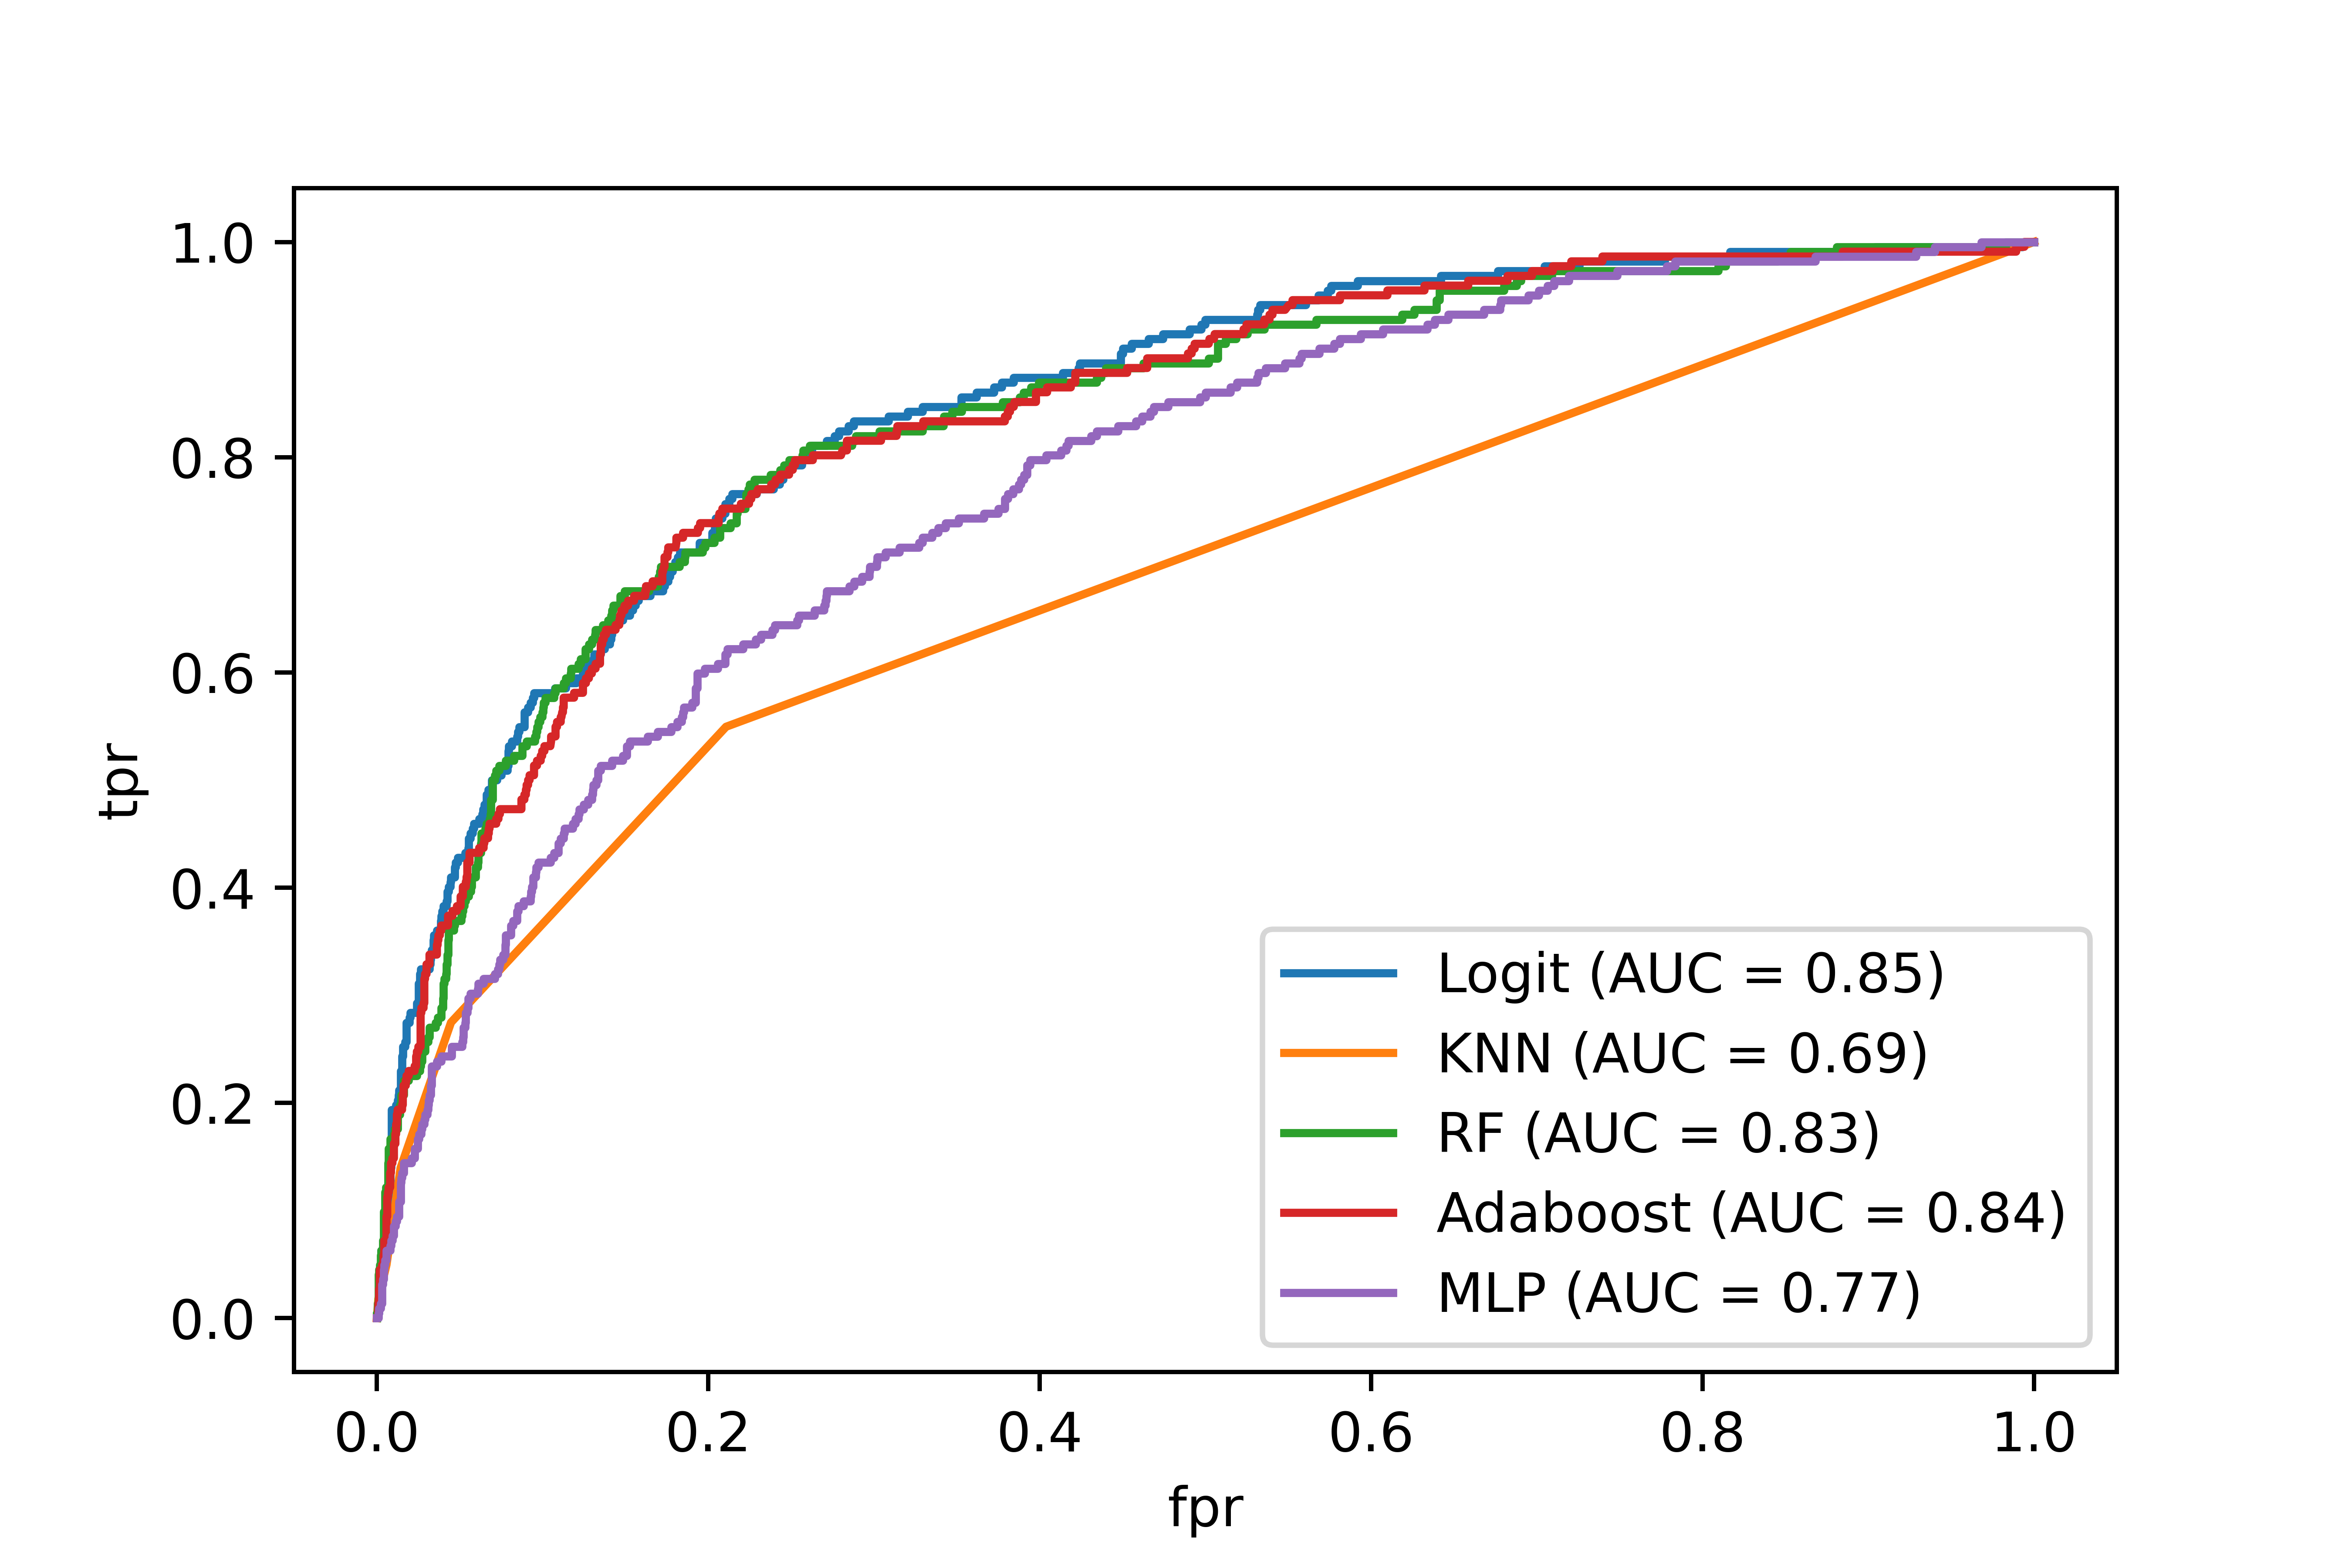
\includegraphics[width=6in]{Pic/ROC_All.png}
\caption{ROC of the 5 models}\label{ROC_All}
\begin{flushleft}{
}\end{flushleft}
\end{figure}

\par In conclusion, the random forest model, the logistic regression model, and the AdaBoost model demonstrated excellent performance in detecting geriatric depression. However, the performance of the KNN model and the MLP model is not satisfying. The problem with the KNN model could be that part of the independent variables are noisy, and the existence of those variables damages the performance of the KNN model. It can be solved by feature selection, such as removing features with low variance, univariate feature selection, and  recursive feature elimination. The problem with the MLP model could be that the structure of the net is not well-tuned. Due to the limitation of computation power, I only considered a small parameter space. A rigorous analysis should search for the optimal parameters in a larger space.

\clearpage
\bibliographystyle{aea}
\bibliography{Mybib}

\clearpage
\vspace{5em}
{\LARGE \bf Appendix:}
% BOX
\begin{figure}[htbp]
\centering
\begin{minipage}[t]{0.48\textwidth}
\centering
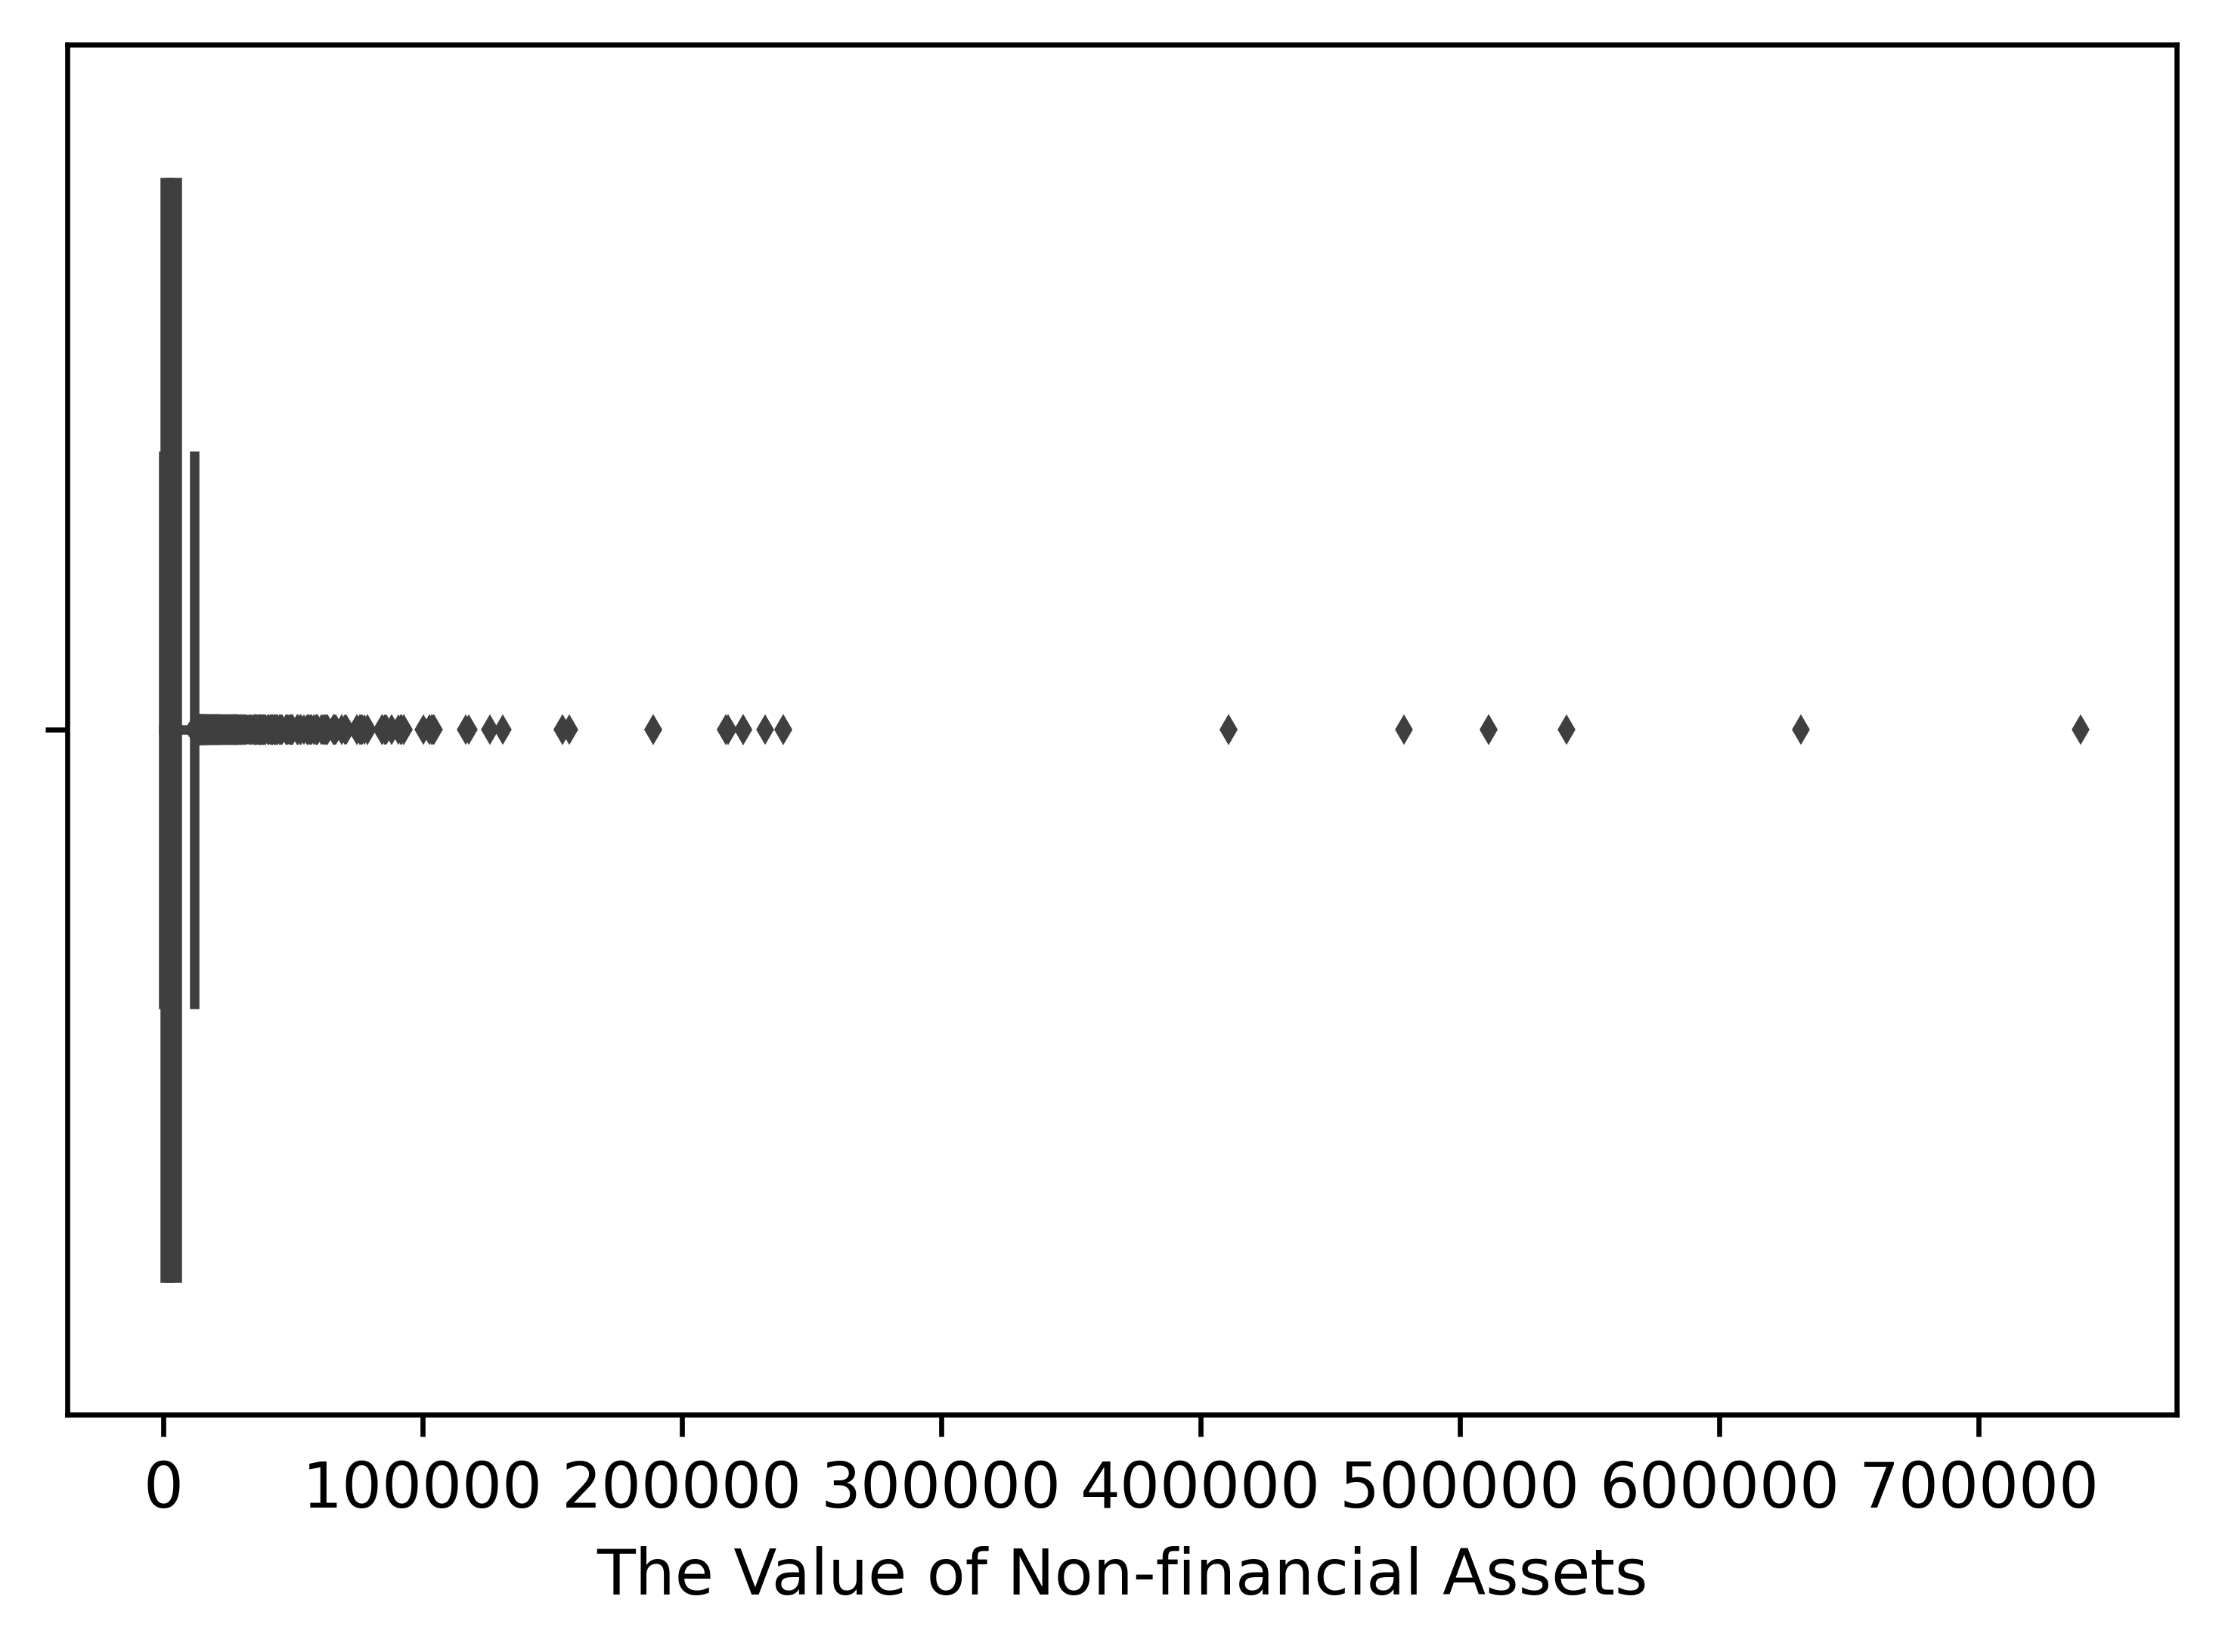
\includegraphics[width=6cm]{Pic/Impute_Durable_Box.png}
\caption{Total Value of Durable Goods}\label{Impute_Durable_Box}
\end{minipage}
\begin{minipage}[t]{0.48\textwidth}
\centering
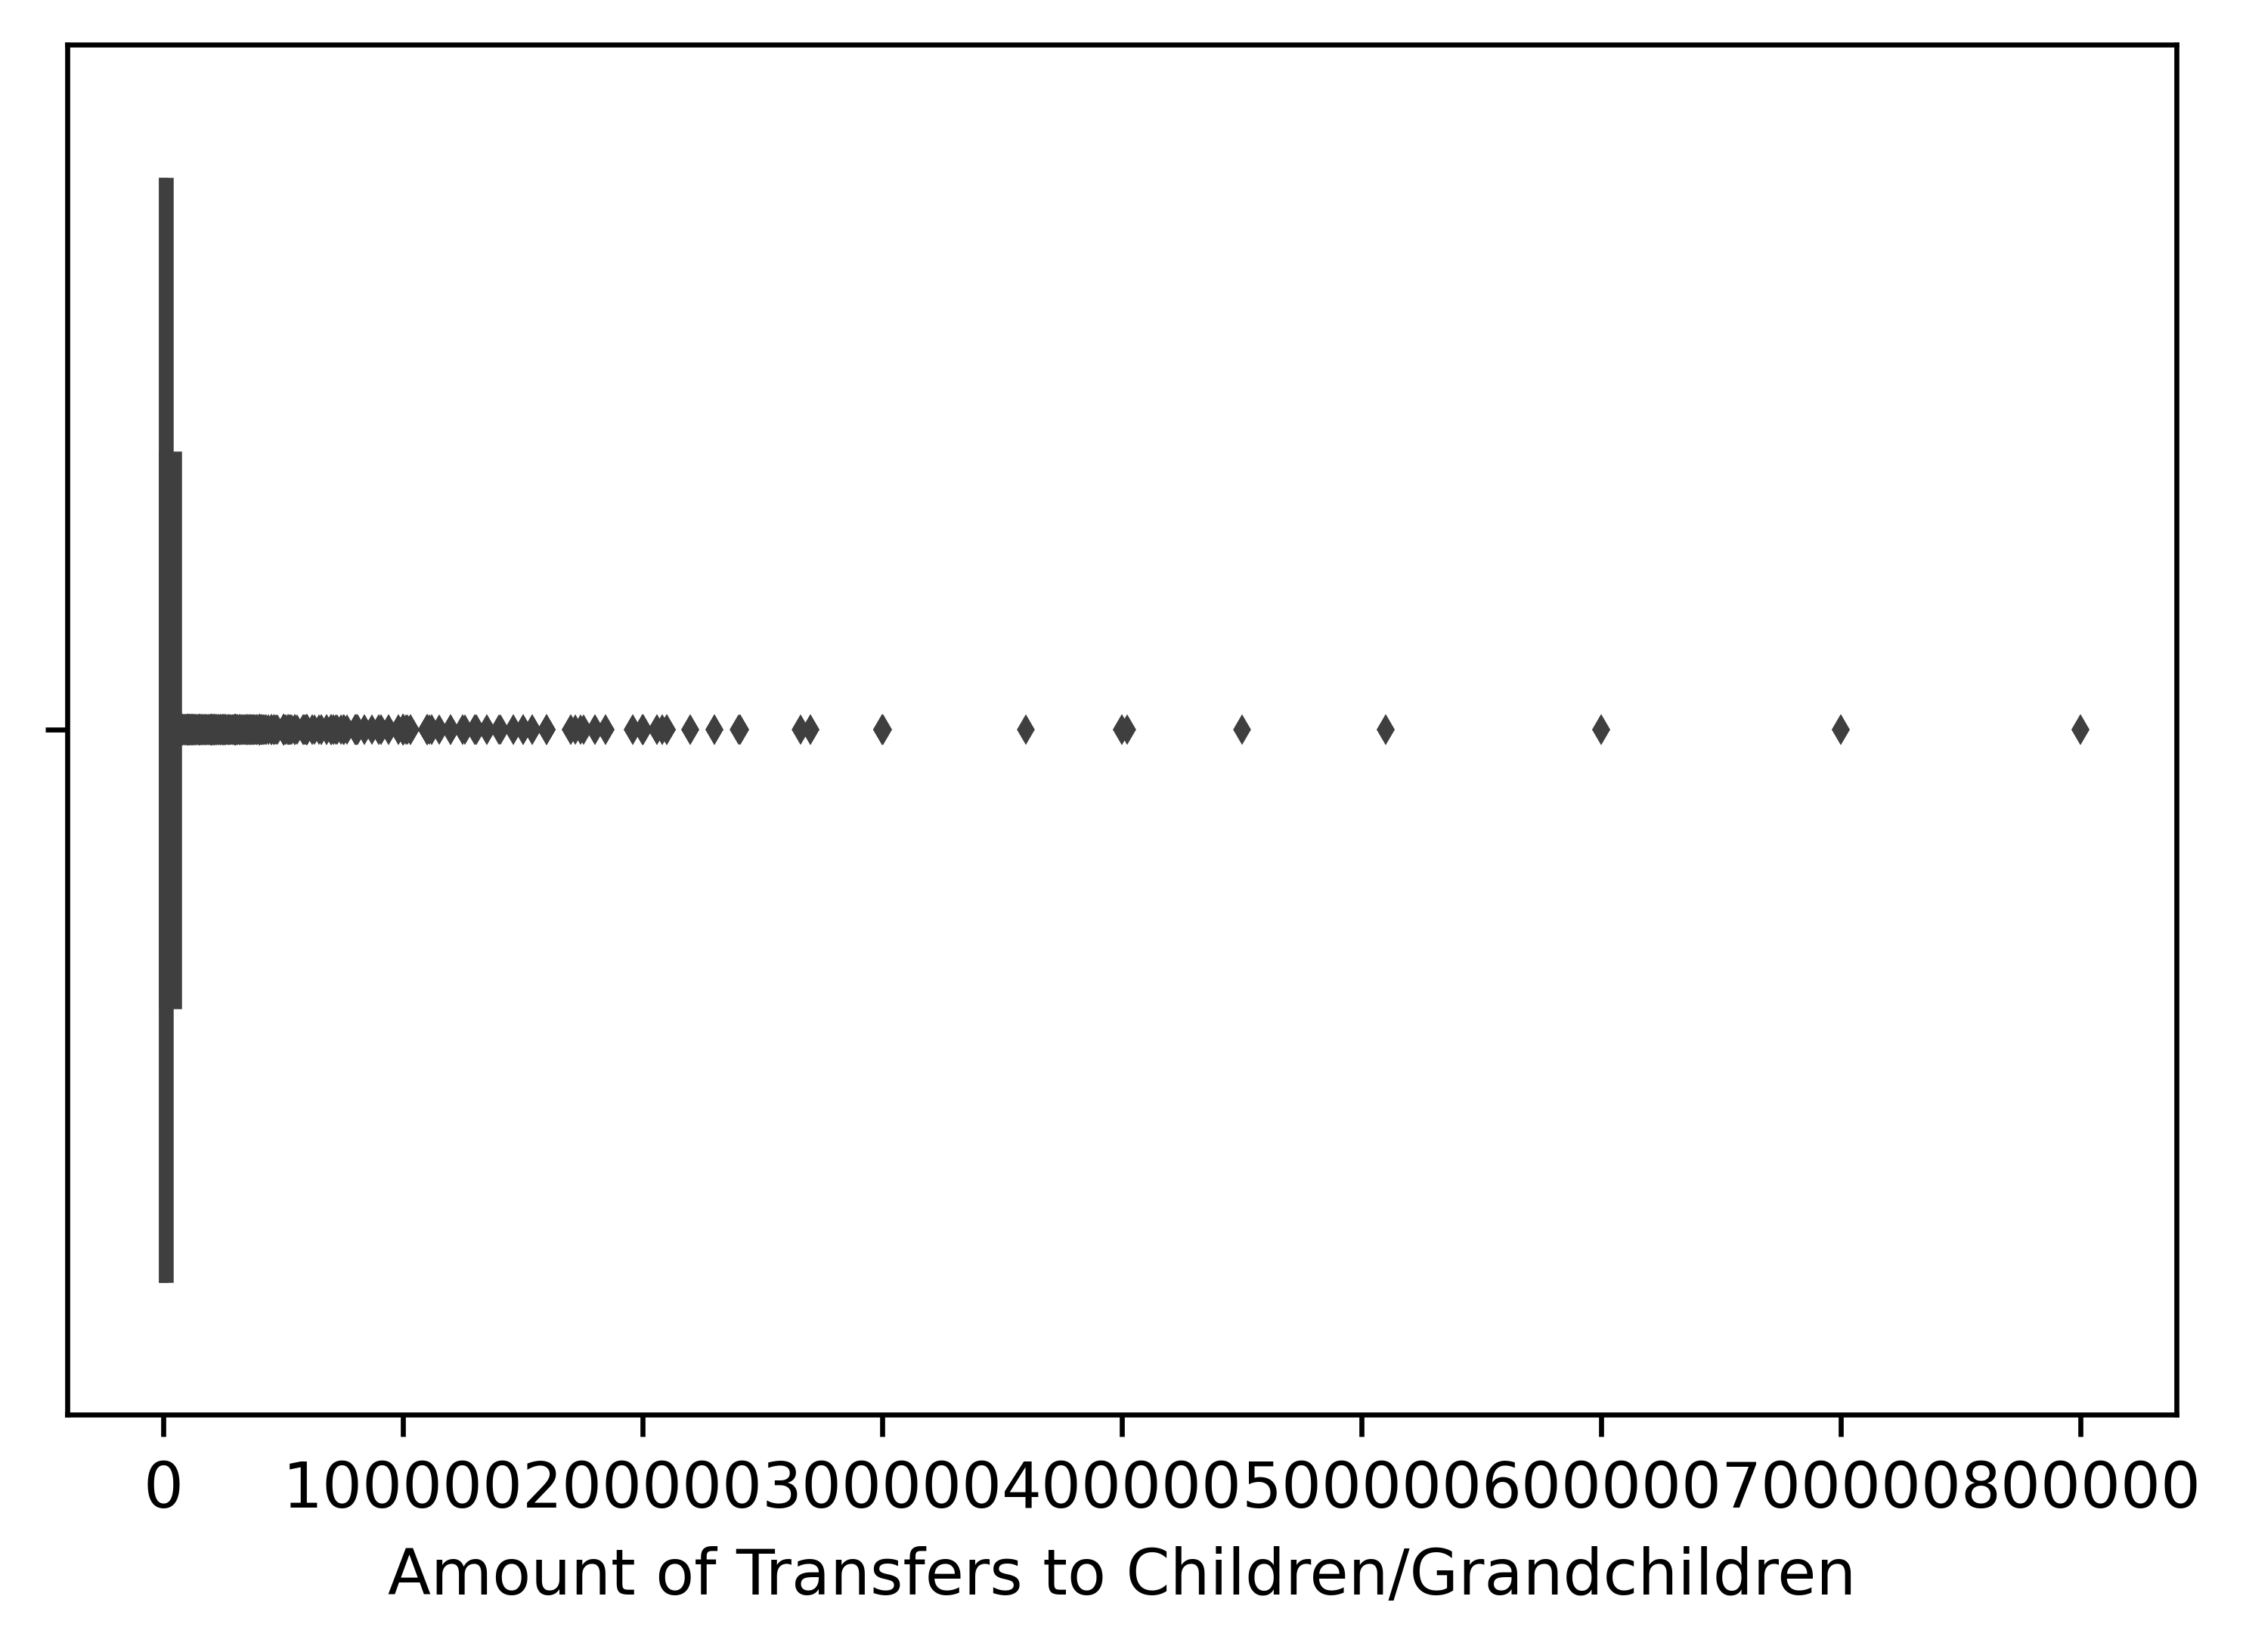
\includegraphics[width=6cm]{Pic/Impute_MoneytChild_Box.png}
\caption{Amount of Money Transferred to Children Last Year}\label{Impute_MoneytChild_Box}
\end{minipage}\\
\begin{minipage}[t]{0.48\textwidth}
\centering
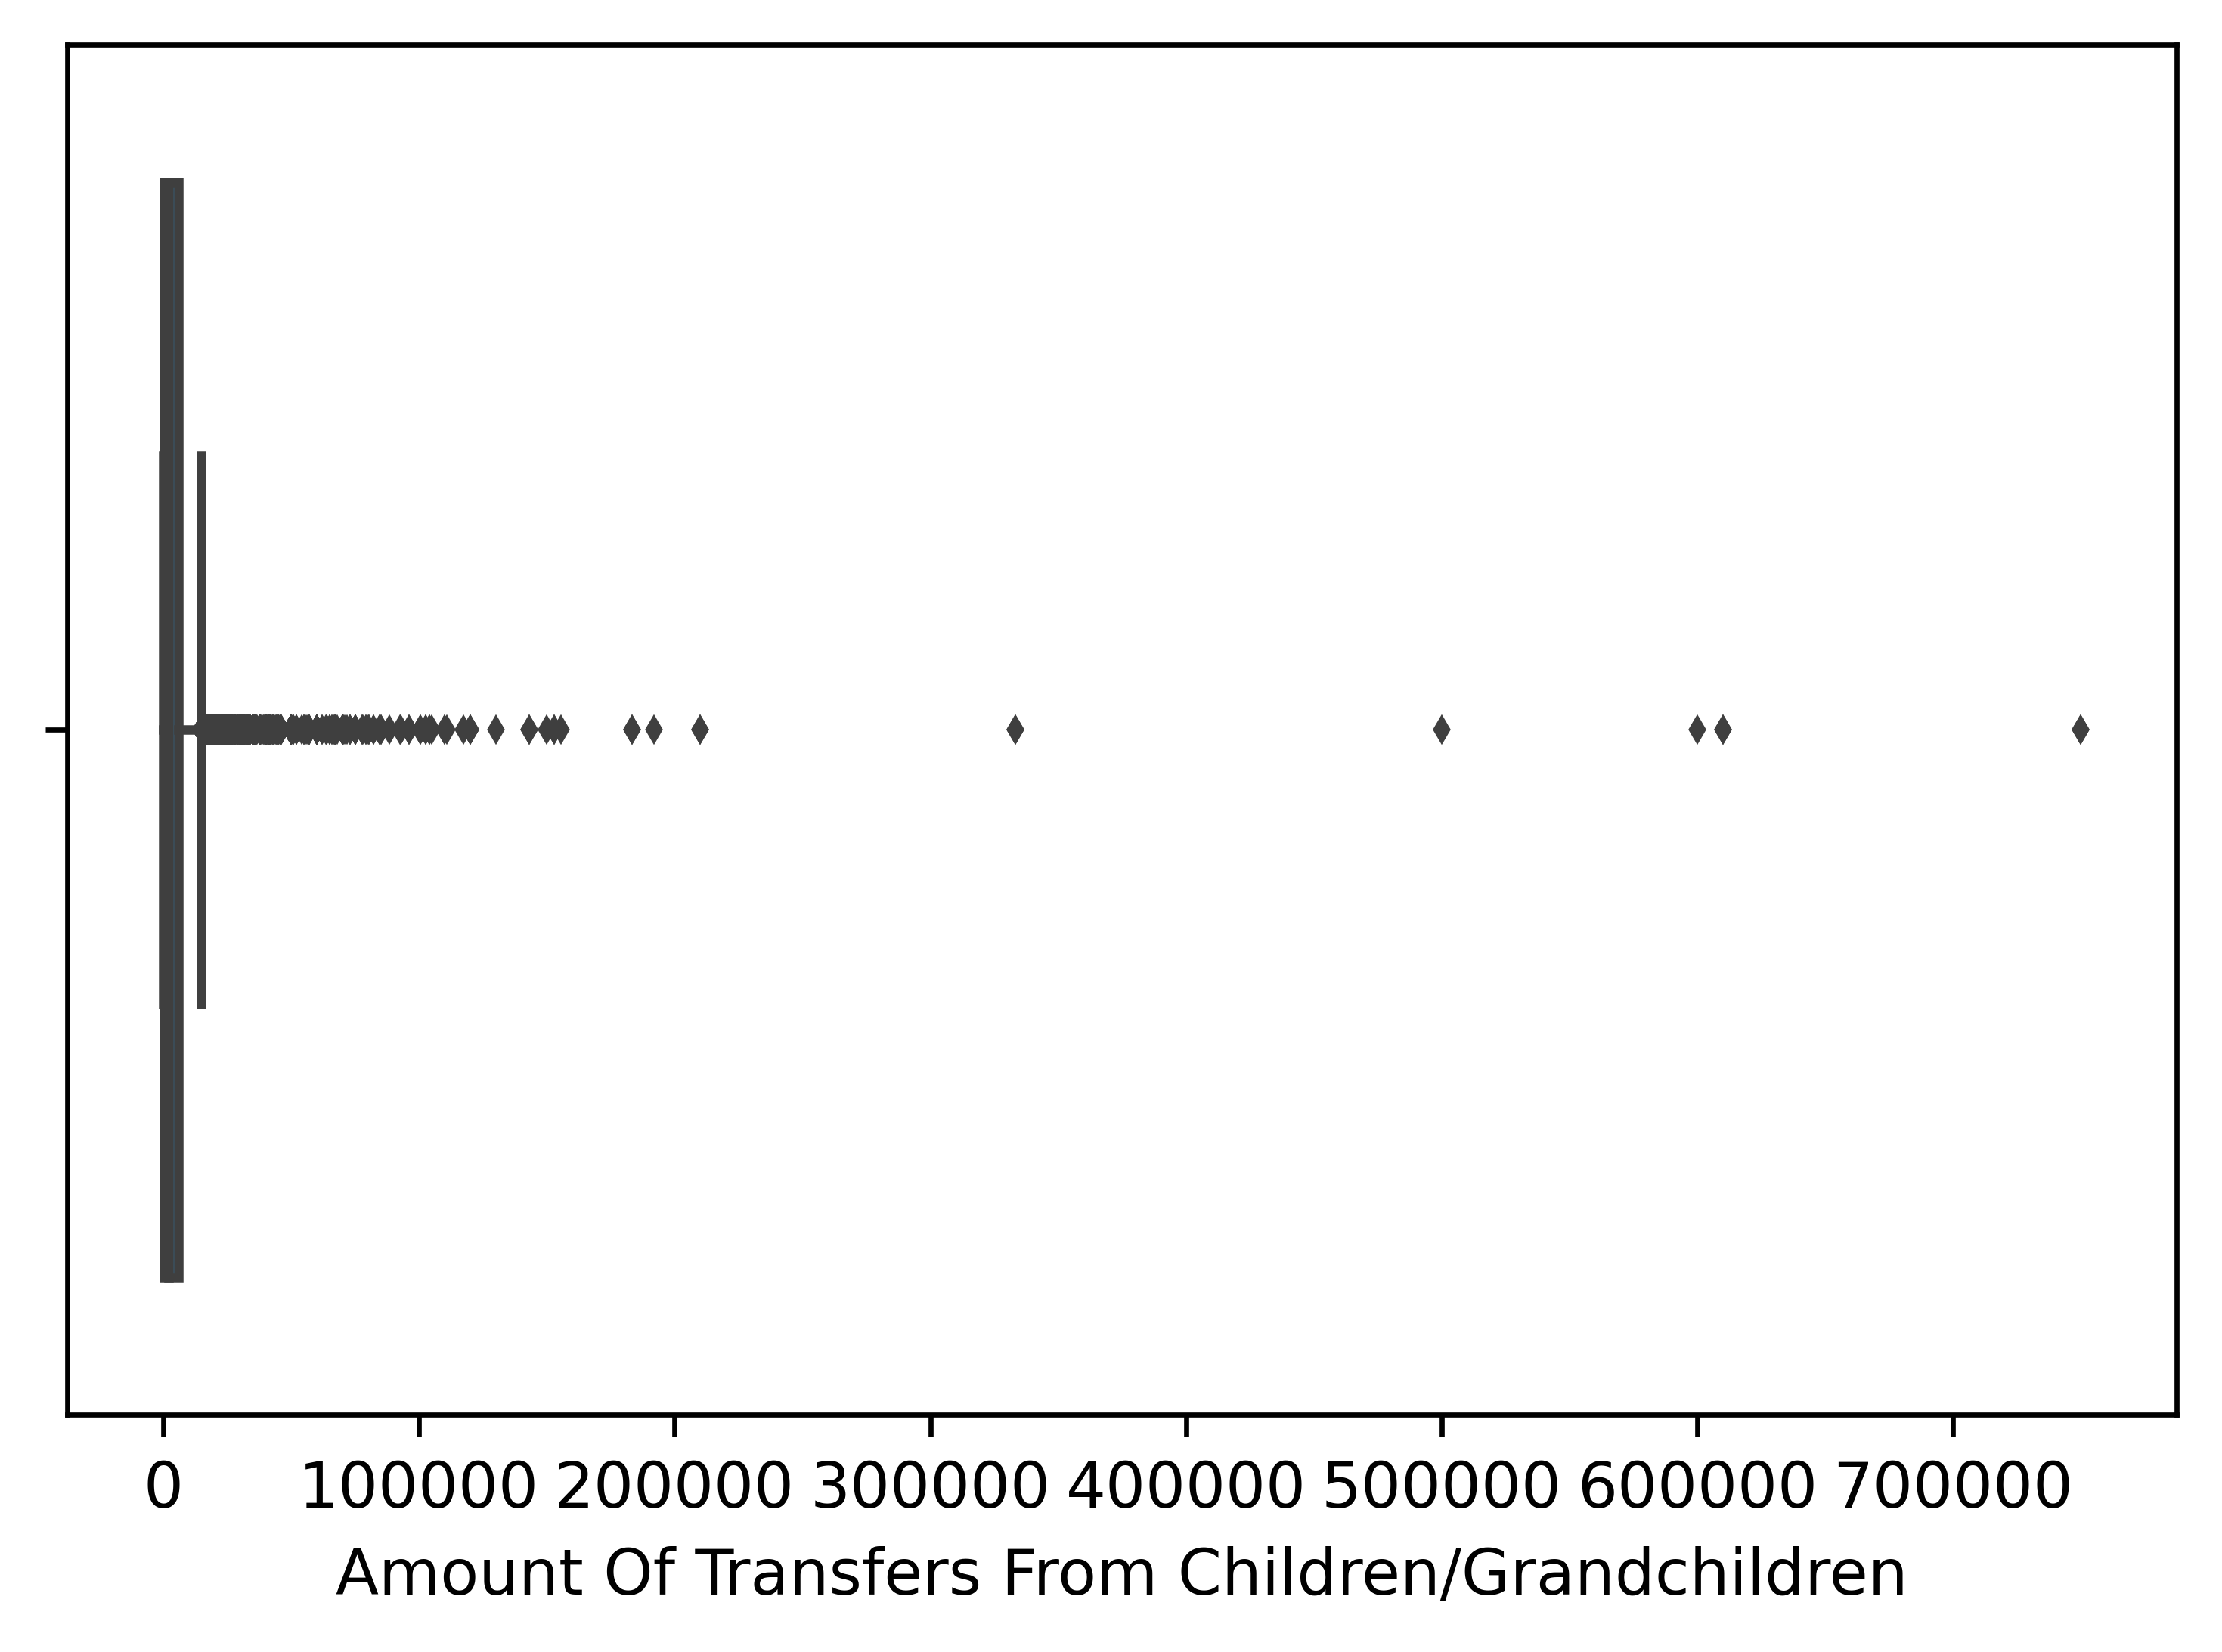
\includegraphics[width=6cm]{Pic/Impute_MoneyfChild_Box.png}
\caption{Amount of Money Received from Children Last Year}\label{Impute_MoneyfChild_Box}
\end{minipage} 
\end{figure}

% Statistics
\begin{table}[htbp]
  \centering
  \caption{Statistic Description} \label{Data_Describe}
     \scalebox{1}{
    \begin{tabular}{lcccccccc}
    \toprule
    \toprule
          & count & mean  & std   & min   & 25\%  & 50\%  & 75\%  & max \\
    \midrule
    Depression & 12283  & 0.09  & 0.29  & 0     & 0     & 0     & 0     & 1  \\
    Male  & 12283  & 0.51  & 0.50  & 0     & 0     & 1     & 1     & 1  \\
    Age   & 12283  & 60.78  & 9.45  & 45    & 52    & 60    & 67    & 100  \\
    Married & 12283  & 0.85  & 0.36  & 0     & 1     & 1     & 1     & 1  \\
    L\_Edu & 12283  & 0.24  & 0.43  & 0     & 0     & 0     & 0     & 1  \\
    M\_Edu & 12283  & 0.63  & 0.48  & 0     & 0     & 1     & 1     & 1  \\
    H\_Edu & 12283  & 0.13  & 0.34  & 0     & 0     & 0     & 0     & 1  \\
    Working & 12283  & 0.68  & 0.47  & 0     & 0     & 1     & 1     & 1  \\
    Rural & 12283  & 0.61  & 0.49  & 0     & 0     & 1     & 1     & 1  \\
    Son   & 12283  & 1.39  & 0.99  & 0     & 1     & 1     & 2     & 7  \\
    Daughter & 12283  & 1.29  & 1.10  & 0     & 1     & 1     & 2     & 9  \\
    Coresd & 12283  & 0.54  & 0.50  & 0     & 0     & 1     & 1     & 1  \\
    HHres & 12283  & 3.06  & 1.35  & 1     & 2     & 3     & 4     & 15  \\
    Durable & 12283  & 4132.29  & 5847.74  & 0     & 700   & 2200  & 5000  & 45800  \\
    MoneytChild & 12283  & 3713.54  & 9443.91  & 0     & 0     & 0     & 2000  & 98000  \\
    MoneyfChild & 12283  & 4686.39  & 6990.84  & 0     & 200   & 2000  & 6000  & 46000  \\
    Province & 12283  & 14.75  & 7.84  & 2     & 9     & 15    & 21    & 31  \\
    Diff\_bath & 12283  & 0.06  & 0.23  & 0     & 0     & 0     & 0     & 1  \\
    Diff\_dress & 12283  & 0.05  & 0.21  & 0     & 0     & 0     & 0     & 1  \\
    Diff\_eat & 12283  & 0.02  & 0.14  & 0     & 0     & 0     & 0     & 1  \\
    Diff\_phone & 12283  & 0.14  & 0.35  & 0     & 0     & 0     & 0     & 1  \\
    Diff\_money & 12283  & 0.08  & 0.27  & 0     & 0     & 0     & 0     & 1  \\
    Diff\_medication & 12283  & 0.04  & 0.18  & 0     & 0     & 0     & 0     & 1  \\
    Smoke & 12283  & 0.29  & 0.45  & 0     & 0     & 0     & 1     & 1  \\
    Alcohol & 12283  & 0.36  & 0.48  & 0     & 0     & 0     & 1     & 1  \\
    Social\_Acti & 12283  & 0.50  & 0.50  & 0     & 0     & 0     & 1     & 1  \\
    Logic & 12283  & 2.79  & 1.97  & 0     & 1     & 2     & 5     & 5  \\
    Memory & 12283  & 6.70  & 3.68  & 0     & 4     & 7     & 9     & 20  \\
    H\_bpressure & 12283  & 0.32  & 0.47  & 0     & 0     & 0     & 1     & 1  \\
    Diabetes & 12283  & 0.09  & 0.29  & 0     & 0     & 0     & 0     & 1  \\
    Cancer & 12283  & 0.02  & 0.13  & 0     & 0     & 0     & 0     & 1  \\
    Lung  & 12283  & 0.14  & 0.35  & 0     & 0     & 0     & 0     & 1  \\
    Heart & 12283  & 0.17  & 0.37  & 0     & 0     & 0     & 0     & 1  \\
    Stroke & 12283  & 0.03  & 0.18  & 0     & 0     & 0     & 0     & 1  \\
    Arthritis & 12283  & 0.41  & 0.49  & 0     & 0     & 0     & 1     & 1  \\
    Dyslipidemia & 12283  & 0.17  & 0.37  & 0     & 0     & 0     & 0     & 1  \\
    Liver & 12283  & 0.06  & 0.24  & 0     & 0     & 0     & 0     & 1  \\
    Kidney & 12283  & 0.09  & 0.29  & 0     & 0     & 0     & 0     & 1  \\
    Digest & 12283  & 0.29  & 0.46  & 0     & 0     & 0     & 1     & 1  \\
    Asthma & 12283  & 0.05  & 0.23  & 0     & 0     & 0     & 0     & 1  \\
    \bottomrule
    \end{tabular}}
\end{table}%

\begin{figure}[htbp]
\centering
\includegraphics[width=6in]{Pic/Demo_Depression-min.png}
\caption{Depression and Demographics}\label{Demo_Depression_Clear}
\end{figure}

\clearpage
\begin{figure}[htbp]
\centering
\includegraphics[width=6in]{Pic/ADL_Depression-min.png}
\caption{Depression and ADL}\label{ADL_Depression_Clear}
\end{figure}

\begin{figure}[htbp]
\centering
\includegraphics[width=6in]{Pic/Diease_Depression-min.png}
\caption{Depression and Diseases}\label{Diease_Depression_Clear}
\end{figure} 

\end{document}